% uid: ""
% school: "college"
% level: "7eme"
% chapter: "التناظر المحوري"
% chapter_slug: "symetrie-axiale"
% title: "الحفاظ على الأطوال والزوايا"
% difficulty: "Facile"
% tags: ["symetrie-axiale", "conservation-longueurs", "conservation-angles", "milieu"]
% provenance: "own"
% batch: "2026-11-27-symetrie-axiale-7eme"
% Exercice 5/10 de la série 7ème « التناظر المحوري » (statement + \axsol + solution). Compiler avec XeLaTeX + axiomath.sty (+ axiomaths-logo.png).
\documentclass[12pt,a4paper]{article}
\usepackage[level=7b,color=0F766E]{axiomath}
\newcommand{\cm}{\,\mathrm{cm}}
\axsetup{title={التناظر المحوري}, corrige}

\begin{document}

\begin{corr}[title={الحفاظ على الأطوال والزوايا}, stars=2, source={Axiomaths}]
$ABC$ مثلث حيث $AB=5\cm$ و $BC=8\cm$ و $AC=7\cm$ و $\widehat{ABC}=60^\circ$. $\Delta$ مستقيم لا يقطع المثلث، و $A'B'C'$ مناظر المثلث $ABC$ بالنسبة إلى $\Delta$.
\begin{enumerate}
  \item احسب $A'B'$ و $B'C'$ و $A'C'$. علّل.
  \item احسب محيط المثلث $A'B'C'$.
  \item ما هو قيس الزاوية $\widehat{A'B'C'}$ ؟
  \item $I$ منتصف $[BC]$ و $I'$ مناظرتها بالنسبة إلى $\Delta$. بين أن $I'$ منتصف $[B'C']$ ، ثم احسب $B'I'$.
\end{enumerate}
\axsol
\begin{enumerate}[itemsep=14pt]
  \item\leavevmode
  \begin{prop}[الحفاظ على الأطوال]
  مناظرة القطعة $[AB]$ هي القطعة $[A'B']$ و \ib{$A'B'=AB$}.
  \end{prop}
  \[A'B'=AB=5\cm\]
  \[B'C'=BC=8\cm\]
  \[A'C'=AC=7\cm\]
  \item محيط $A'B'C'$ هو مجموع أطوال أضلاعه :
  \[5+8+7=20\cm\]
  وهو نفس محيط $ABC$.
  \item\leavevmode
  \begin{prop}[الحفاظ على قيس الزوايا]
  مناظرة زاوية بالنسبة إلى مستقيم هي \ib{زاوية لها نفس القيس}.
  \end{prop}
  الزاوية $\widehat{A'B'C'}$ مناظرة الزاوية $\widehat{ABC}$ ، إذن :
  \[\widehat{A'B'C'}=\widehat{ABC}=60^\circ\]
  \item\leavevmode
  \begin{prop}[الحفاظ على المنتصف]
  مناظرة منتصف قطعة هي \ib{منتصف القطعة المناظرة}.
  \end{prop}
  $I$ منتصف $[BC]$ ، و $[B'C']$ مناظرة $[BC]$ ، إذن \ib{$I'$ منتصف $[B'C']$}.
  \[B'I'=\dfrac{B'C'}{2}=\dfrac{8}{2}=4\cm\]
  \begin{center}
  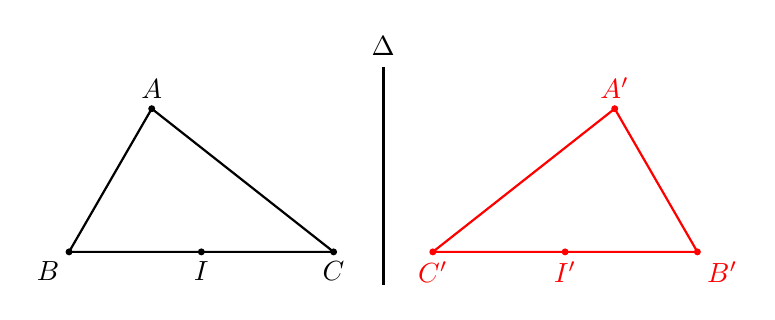
\begin{tikzpicture}[scale=0.42]
    \draw[very thick] (9.5,-1)--(9.5,5.6) node[above] {$\Delta$};
    \draw[thick] (0,0)--(8,0)--(2.5,4.330)--cycle;
    \draw[thick,red] (19,0)--(11,0)--(16.5,4.330)--cycle;
    \fill (0,0) circle (3pt) node[below left] {$B$};
    \fill (8,0) circle (3pt) node[below] {$C$};
    \fill (2.5,4.330) circle (3pt) node[above] {$A$};
    \fill (4,0) circle (3pt) node[below] {$I$};
    \fill[red] (19,0) circle (3pt) node[below right] {$B'$};
    \fill[red] (11,0) circle (3pt) node[below] {$C'$};
    \fill[red] (16.5,4.330) circle (3pt) node[above] {$A'$};
    \fill[red] (15,0) circle (3pt) node[below] {$I'$};
  \end{tikzpicture}
  \end{center}
\end{enumerate}
\end{corr}

\end{document}
